% -*- coding: utf-8 -*-
% !TEX encoding = UTF-8 Unicode
% !TEX root =  main.tex

\chapter{Beispiel Kapitel}
\label{chap:beispiel-kapitel}

Eine Abbildung lässt sich einfach über:

\lstset{language=TeX}
\begin{lstlisting}

\begin{figure}[htb]
\centering
\includegraphics[width=\textwidth]{_images/chapter1/foc-ac-dc.pdf}
\caption{Beschriftung der Abbildung}
\label{fig:foc-ac-dc}
\end{figure}

\end{lstlisting}

einfügen.
Die breite der Abbildung kann einerseits skaliert oder direkt im Maßstab von \SI{14.5}{\centi\meter} erstellt werden.
Wenn die Abbildung maßstabsgetreu erstellt wird, muss \verb|\centering| und der optionale Befehl \verb|[width=\textwidth]| nicht zwingend übernommen werden.

\begin{figure}[htb]
	\centering
	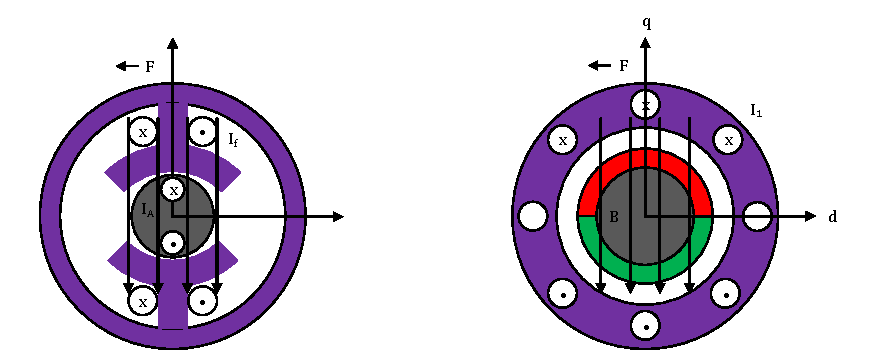
\includegraphics[width=\textwidth]{foc-dc-ac.pdf}
	\caption{Beschriftung der Abbildung}
	\label{fig:foc-dc-ac}
\end{figure}

Für Zitationen wird \verb|BibLaTeX| verwendet. Als Backend wird \verb|biber| vom Kompiler verlangt.
Biber ist Open Source und kann im CTAN Repository heruntergeladen werden: \url{https://www.ctan.org/pkg/biber}.

\begin{quote}
\enquote{Bei jeder permanentmagneterregten Synchronmaschine ändern sich die Induktivitäten in abhängigkeit von der Last. In erster Linie sind dafür die Sättigungseffekte, aber auch die Kreuzkopplung verantwortlich.} \autocite[S.~2]{ternes2015}
\end{quote}

Im Text zitierte Werke werden über die Syntax \verb|\textcite[S.~2]{ternes2015}| korrekt zitiert. Beispielsweise: Wie in \textcite[S.~2]{ternes2015} erläutert, sind die Induktivitäten abhängig von der Last \ldots

Der aktuelle Stil des Literaturverzeichnisses und der Zitationen ist \verb|alphabetic|, kann aber auch in Absprache geändert werden, dazu empfiehlt es sich, die \verb|BibLaTeX|-Dokumentation zu konsultieren.

%%% Local Variables: 
%%% mode: latex
%%% TeX-master: "main"
%%% TeX-open-quote: "\\enquote{"
%%% TeX-close-quote: "}"
%%% LaTeX-csquotes-open-quote: "\\enquote{"
%%% LaTeX-csquotes-close-quote: "}"
%%% End: 
